\section{Data Preparation}

\subsection{Defining the Target Variable}
Our goal is to enhance and automate the triage process for patients arriving at the hospital diagnosed with COVID-19. Implementing an 
automated triage system, we aim to streamline the initial assessment
and quickly determine the appropriate level of care required for 
each patient. The outcome of this automated system will
categorize patients into one of three categories:

\begin{description}
\item[Maybe] This outcome is indeterminate, suggesting that the 
case isn't clear-cut. Such patients might need further analysis 
either through a follow-up assessment after some time or an 
immediate review by a medical professional.
\item[No] Indicates that the patient does not require hospitalization. 
These patients are stable enough to be sent home with 
instructions for self-care and possibly follow-up recommendations.
\item[Yes] Signifies that the patient requires hospital 
admission due to the severity of their symptoms or
underlying health conditions that pose increased risk.
\end{description}

By classifying incoming patients into these categories, the hospital 
can reduce contact with front line medical staff as well as optimize 
resource allocation and reduce wait times. 
This system not only enhances operational efficiency but also 
improves patient outcomes by facilitating immediate and accurate
decision-making at the point of entry~\footnote{You can find the 
transformation details in the function 
\texttt{makeRequiredTreatment} in the Listing~\ref{lst:feat_norm_functions}}.

The target variable prediction is true if the following conditions are
true in the dataset:

\begin{table}[H]
    \centering
    \caption{Hospitalization Patient Required Condition Rules}
    \label{tab:target_variable_rules}
    \begin{tabular}{ccccc} \hline
     \textbf{Patient Type} & \textbf{ICU} & \textbf{Intubed} & \textbf{Died} & \textbf{Required Treatment}\\ 
     \hline \hline
      NA & NA & NA & Yes~($\neq 9999-99-99$) & Yes \\
      NA & NA & Yes~($1$) & No~($= 9999-99-99$) & Yes \\ 
      NA & Yes~($1$) & NA & No~($= 9999-99-99$) & Yes \\
      Home~($1$) & No & NA & No~($= 9999-99-99$) & No \\
      Hospitalized~($1$) & NA & NA & No~($= 9999-99-99$) & Maybe \\ \hline
    \end{tabular}
\end{table}

\subsection{Data Normalization}
This dataset includes numerous binary variables, each encoded 
with distinct meanings. We found these hard to reason about when
analysing the data so we converted them to short text values.
While we considered using 
the \emph{Edit Domain Widget}~\parencite[]{2015:odm} from
\emph{Orange Data Mining} as cited in , we found the task to be 
cumbersome, involving considerable repetition, and challenging in terms of 
replicating the logic applied previously (Figure~\ref{fig:data_preparation_edit_domain} 
and Figure~\ref{fig:data_preparation_using_formula}). 

Instead, we utilized a Scala Script (Listing~\ref{lst:feat_norm_functions} and Listing~\ref{lst:feat_norm_process}) that reads the original dataset 
and transforms the data as follows:

\begin{table}[H]
    \centering
    \caption{Feature Normalization}
    \label{tab:feat_normalization}
    \begin{tabular}{cc} \hline 
     \textbf{Feature} & \textbf{Transformation} \\ \hline\hline
      sex &  $1 \to female$, $2 \to male$ \\ 
      age &  \\ 
      classification &  \\ 
      patientType & $1 \to home$, $2 \to hospital$ \\ 
      pneumonia & $1 \to yes$, $2 \to no$ \\ 
      pregnancy & $sex = female \land 1 \to yes$, $sex = female \land 2\to no$, $sex = male \to na$ \\
      diabetes & $1 \to yes$, $2 \to no$ \\ 
      copd & $1 \to yes$, $2 \to no$ \\ 
      asthma & $1 \to yes$, $2 \to no$ \\ 
      inmsupr & $1 \to yes$, $2 \to no$ \\ 
      hypertension & $1 \to yes$, $2 \to no$ \\ 
      cardiovascular & $1 \to yes$, $2 \to no$ \\ 
      renal\_chronic & $1 \to yes$, $2 \to no$ \\ 
      other\_disease & $1 \to yes$, $2 \to no$ \\ 
      obesity & $1 \to yes$, $2 \to no$ \\
      tobacco & $1 \to yes$, $2 \to no$ \\
      usmer & \\
      medical\_unit & \\
      intubed & $1 \to yes$, $2 \to no$ \\ 
      icu & $1 \to yes$, $2 \to no$ \\ 
      date\_died & $9999-99-99 \to no$, $otherwise \to yes$\\ \hline 
    \end{tabular}
\end{table}

\subsection{Feature Removal}
To streamline our model for predicting hospitalization
requirements, we have decided to create a target variable named 
`Required Hospitalization.' Consequently, any features used to
construct `Required Hospitalization` will be excluded from the 
predictive modeling phase and reserved solely
for the verification process:
\begin{itemize}
    \item Patient Type;
    \item Intubed;
    \item ICU;
    \item Date Died.
\end{itemize}

By removing these features from the modeling stage, we ensure that the 
model develops the ability to predict hospitalization based on less direct
indicators, thereby enhancing its applicability and effectiveness in 
real-world triage scenarios.

A medical unit is typically composed of a team of doctors and nurses operating within a larger 
entity, such as the armed forces, a prison, or a hospital. Given this definition, we conclude that
the presence of a medical unit does not directly influence the decision regarding a patient's need 
for hospitalization. Therefore, we have decided to exclude the \texttt{MEDICAL\_UNIT} feature from 
our analysis.

The variable \texttt{USMER}\footnote{\texttt{USMER} refers at which type a patient
received in a medical unit.} was removed from our analysis because it indicates whether
a patient was hospitalized, making it a consequence rather than a predictor. Including
it could potentially bias our predictive modeling efforts, as it does not contribute
to determining the factors leading to hospitalization but rather describes an outcome.
Thus, to maintain the integrity of our model and ensure it accurately identifies true 
predictive variables, \texttt{USMER} has been excluded.

So in summary we also remove the following features:
\begin{itemize}
    \item Medical Unit;
    \item USMER.
\end{itemize}


\subsection{Outliers}

We have 208 cases of patients aged between 100 and 121 years. It seems 
improbable to have such a high number of patients over 104 years old. However,
since these cases only represent 208 out of 1 million and are likely to be 
older patients, we believe this data will not significantly impact the final 
calculations.

\begin{figure}[H]%
    \caption{Age >= 100 Years old}%
    \label{fig:data_preparation_edit_domain}%
    \centering
    {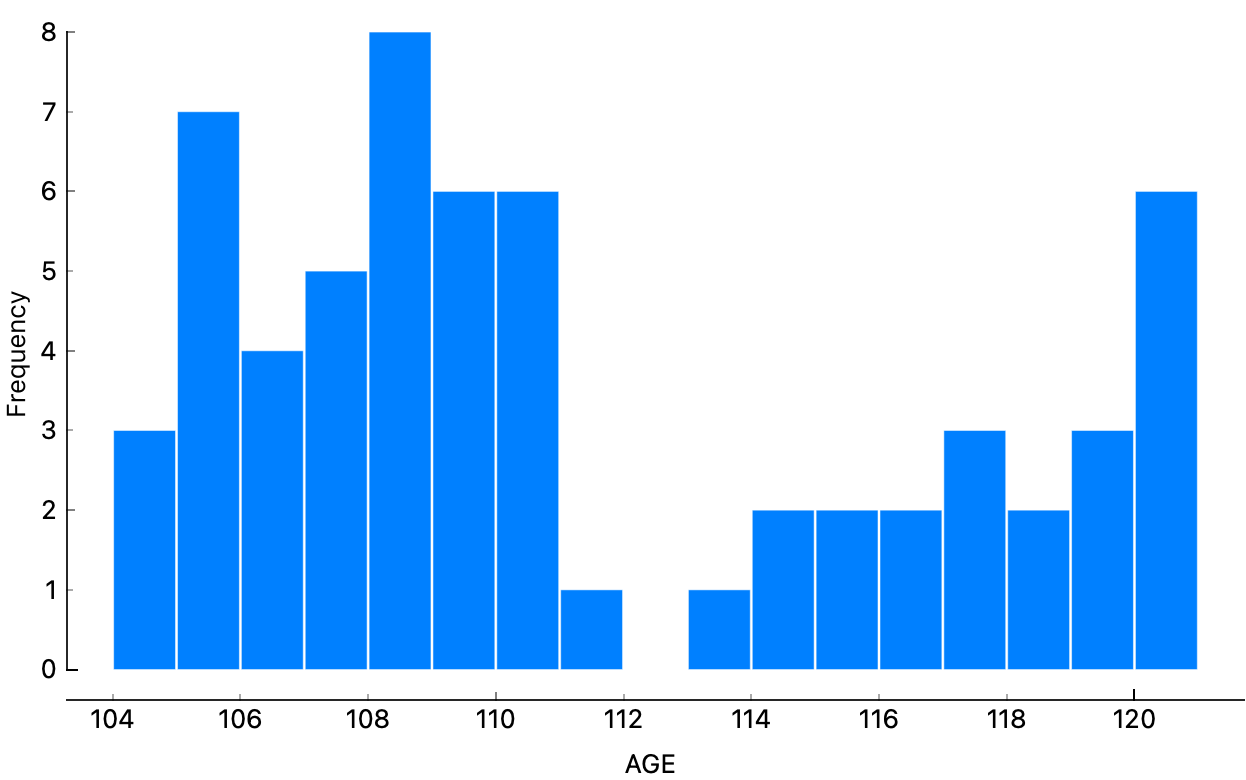
\includegraphics[width=\textwidth]{img/dataexploration/outliers_age.png} }
\end{figure}

\subsection{Missing Values}

In the dataset we're discussing, most of the features are quite
complete, with each having about 3,000 missing entries. Despite
this, these missing entries only account for a negligible 
portion of the entire dataset—essentially 0\% of all the data, 
indicating that the overall impact on the dataset's integrity 
is minimal.

However, one particular feature, `pregnancy status' stands 
out due to a higher rate of missing data. This feature is 
missing 50\% of its values. The reason for this significant 
number of missing values is linked to the data normalization
process. Specifically, the data entries related to males are 
marked as missing in the pregnancy status field, because 
pregnancy is not applicable to them.

Additionally, the feature for pneumonia has a 2\% rate of 
missing values from the sample data. Given this relatively low
proportion of missing data, we plan to impute these missing
entries with the most common response, which is `no'. This 
approach is justified by the high likelihood -- 87\% -- that a
given entry would not have pneumonia, based on the data we 
have. 

\subsection{Feature Selection}

Because we have only 14 Features we won't apply any dimension 
reduction but we can still identify the most relevant features
for the target variable. This is a important step because we can
verify if our training models will pick the most important
variables to classify the patients that needs to be hospitalized.

In the article by Jason Brownlee~\parencite[]{2020:brownlee}, it is suggested 
that when dealing with a large number of 
categorical variables, the most 
effective metrics to assess their importance
are \emph{Chi-Squared Statistics} 
($\chi^2$)
and \emph{Information Gain}. These metrics are particularly useful for 
identifying which variables have the strongest 
relationships with the target 
variable, thereby helping to refine and improve the 
performance of predictive 
models. The Figure~\ref{fig:feat_rank_5} shows the top $\chi^2$ ranked
variables\footnote{The full ranked variables ranking are in 
Figure~\ref{fig:feat_full_rank}.}.

\begin{figure}[H]%
    \caption{Top 5 Ranked Features for predicting if a Patient needs Hospitalization}%
    \label{fig:feat_rank_5}%
    \centering
    {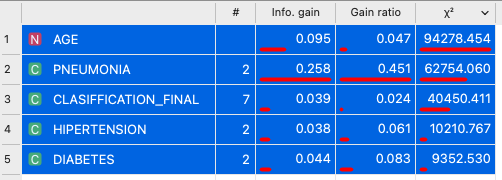
\includegraphics[width=0.6\textwidth]{img/datapreparation/feat_rank_5.png} }
\end{figure}

\subsection{Dimension Reduction}

We have decided not to apply any dimension reduction 
techniques to train the data due to several key reasons:
\begin{description}
    \item[Categorical Variables]: Our dataset consists 
    predominantly of categorical variables, which do not lend 
    themselves well to traditional dimension reduction 
    techniques like PCA that are better suited for continuous 
    data;
    \item[Interpretability]: Dimension reduction can often 
    obscure the meaning of the original variables. Given the 
    importance of each variable in our dataset for clinical 
    decision-making and understanding patient outcomes, 
    maintaining the interpretability of the data is crucial.
    Reducing variables like Tobacco, Obesity, Diabetes or 
    Pneumonia or Age will contribute for lack of understanding
    of the outcomes;
    \item[Complex Relationships]The relationships between 
    variables in our dataset are complex and may not be 
    linear. Dimension reduction techniques, particularly 
    those based on linear assumptions, might not capture 
    these nuances effectively, leading to sub-optimal
    model performance.
\end{description}

Considering we only have 15 features that are crucial for the 
training and explainability of the model's outcomes, we have 
decided not to reduce any features for training. This decision 
stems from a few key points:
\begin{description}
    \item[Importance] Each feature has been identified as 
    significant in impacting the model’s predictions. Removing 
    any of these could jeopardize the accuracy and reliability 
    of the model;
    \item[Dataset] With just 15 features, our dataset is 
    relatively concise. This manageable number of features 
    facilitates a straightforward training process and clear
    interpretation of results, making further reduction 
    unnecessary.
\end{description}
    
\subsection{Dataset Isolation}

To enhance our model's effectiveness we have divided the dataset
as detailed in the Table~\ref{tab:dataset_split}. This 
division is aimed at preventing
the model from merely training the data avoiding overfitting. 
Isolating the data also ensures that the model remains robust
across various data samples (Not merely the ones on which it
was trained.). Splitting the data also facilitates a fair 
evaluation. As assessing the model on previously unseen data
yields more accurate results and better reflects real-world
scenarios. 

\begin{table}[H]
    \centering
    \caption{Splitting the Data}
    \label{tab:dataset_split}
    \begin{tabular}{ccp{10cm}} \hline
     \textbf{Dataset} & \textbf{Size} & \textbf{Comment} \\ \hline\hline
      Trainning & 692060 (66\%) & This is the largest portion of
      the data and is used to train
      the model. The model learns to recognize patterns and make decisions based on 
      this dataset. \\
      Verification & 235300 (22\%) & The validation set is used to tune
      the hyperparameters of 
      the model and prevent overfitting. It acts as a check during training to
      ensure that the model not only learns the training data well but can also 
      apply this learning to new data. It is used to evaluate model performance 
      during the training process. \\ 
      Testing & 121215 (12\%) & After the model has been trained and validated, the test
      set is used to assess its performance. This data set is never used in the 
      training phase and serves as a new, unbiased platform to evaluate how well the 
      model can generalize its learning to data it has never seen before. \\ \hline
    \end{tabular}
\end{table}

To split the data we used the 
\emph{Orange Data Mining Data - Sampler Widget} (Figure~\ref{fig:data_preparation_splitting}) with the 
options:
\begin{itemize}
    \item Replicable (deterministic) sampling;
    \item Stratify sample (when possible).
\end{itemize}

The Replicable sampling ensures that sampling patterns can be consistently applied
across different users.

Stratified splitting ensures that each division of the dataset accurately 
reflects the overall dataset in terms of key characteristics' proportions. 
This approach is particularly crucial for handling imbalanced datasets.

\begin{figure}[H]%
    \caption{Orange Data Mining Data Splitting}%
    \label{fig:data_preparation_splitting}%
    \centering
    {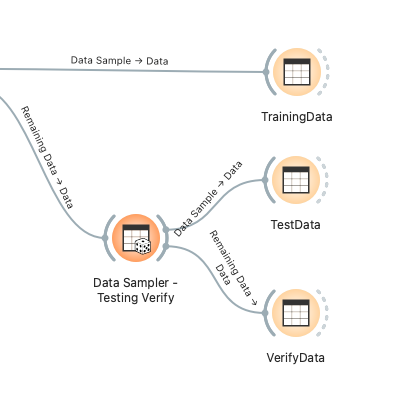
\includegraphics[width=0.6\textwidth]{img/datapreparation/datapreparation_splitting.png} }
\end{figure}

